\Aufgabe[e]{Drehmatrizen}{
Eine Matrix der Form
$$
\boldsymbol A = 
\begin{pmatrix}
\cos \alpha  & -\sin \alpha  \\
\sin \alpha  &  \cos \alpha
\end{pmatrix}
$$
beschreibt eine Drehung eines Vektors um den Winkel $\alpha$.

Gegeben seien die Vektoren
$$
\boldsymbol v =
\begin{pmatrix}
2 \\ 1
\end{pmatrix}\,\, , \,\,
\boldsymbol w = 
\begin{pmatrix}
-1 \\ 1
\end{pmatrix}.
$$
\begin{abc}
\item
Bestimmen Sie die Euklidische Norm von $\boldsymbol v$ und $\boldsymbol w$
und skizzieren Sie die beiden Vektoren.
\item 
Bestimmen Sie jeweils die Matrix-Vektor-Produkte $\boldsymbol A \boldsymbol v$
und $\boldsymbol A \boldsymbol w$ für die Winkel $\alpha = \frac{\pi}{2}$ und 
$\beta = -\frac{\pi}{3}$. 
\item
Skizzieren Sie die Ergebnisvektoren und bestimmen Sie jeweils die Euklidische Norm.
\end{abc}
}
\Loesung{
\begin{abc}
\item
Die Normen der gegebenen Vektoren sind
$$
\| \boldsymbol v \|_2 = \sqrt{2^2+1^2} = \sqrt{5} \quad , \quad  
\| \boldsymbol w \|_2 = \sqrt{(-1)^2+1^2} = \sqrt{2}
$$
\item
Für den Winkel $\alpha = \frac{\pi}{2}$ ist die Matrix
$$
\boldsymbol A =
\begin{pmatrix}
 0 & -1 \\
 1 &  0
\end{pmatrix}
$$
Die Matrix-Vektor-Produkte sind
$$
\boldsymbol A \boldsymbol v = 
\begin{pmatrix}
-1 \\ 2
\end{pmatrix} \quad , \quad
\boldsymbol A \boldsymbol w = 
\begin{pmatrix}
-1 \\ -1
\end{pmatrix}.
$$

Für den Winkel $\beta = -\frac{\pi}{3}$ ist die Matrix
$$
\boldsymbol B =
\frac{1}{2}
\begin{pmatrix}
 1 & \sqrt{3} \\
 -\sqrt{3} &  1
\end{pmatrix}
$$
Die Matrix-Vektor-Produkte sind
$$
\boldsymbol B \boldsymbol v = 
\frac{1}{2}
\begin{pmatrix}
 2+\sqrt{3} \\ -2\sqrt{3}+1
\end{pmatrix} \quad , \quad
\boldsymbol B \boldsymbol w = 
\frac{1}{2}
\begin{pmatrix}
 -1 +\sqrt{3} \\ 1+\sqrt{3}
\end{pmatrix}.
$$
\item
$$
\| \boldsymbol Av \|_2 = \sqrt{5} \quad , \quad  
\| \boldsymbol Aw \|_2 = \sqrt{2} 
$$
$$
\| \boldsymbol Bv \|_2 = \sqrt{5} \quad , \quad  
\| \boldsymbol Bw \|_2 = \sqrt{2} 
$$
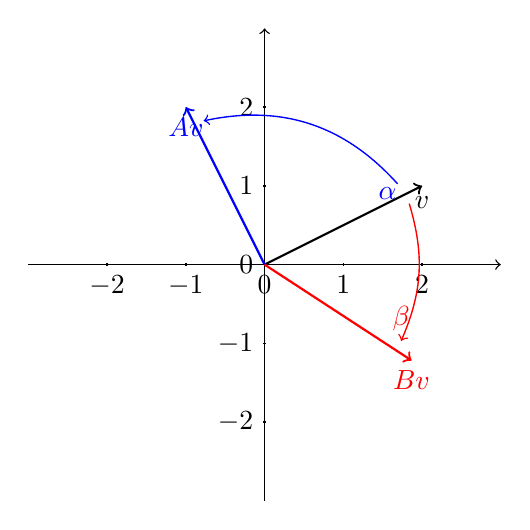
\begin{tikzpicture} [scale=0.5,line width=0.5]
%%%%%%%%%%	Koordinaten	%%%%%%%%%%
\foreach \x in {-2,...,2}
    \draw (2*\x cm,1pt) -- (2*\x cm,-1pt) node[anchor=north] {$\x$};
\foreach \y in {-2,...,2}
    \draw (1pt,2*\y cm) -- (-1pt,2*\y cm) node[anchor=east] {$\y$};

    \draw[->] (-6,0) -- (6,0);
    \draw[->] (0,-6) -- (0,6);

    \draw[->,thick] (0,0) -- (4,2) node[anchor = north] {$\boldsymbol v$};
    \draw[->,blue,thick] (0,0) -- (-2,4) node[anchor = north] {$\boldsymbol A \boldsymbol v$};
    \draw[->,red,thick] (0,0) -- (3.732,-2.434) node[anchor = north] {$\boldsymbol B \boldsymbol v$};
    \node (A) at (3.6,1.8){};
	\node (B) at (-1.8,3.6){};
	\node (C) at (3.359,-2.191){};
	
	\draw[->,blue] (A)node[blue,anchor = east] {$\alpha$} to [bend right = 30] (B) ;
	\draw[->,red] (A) to [bend left = 20] (C) node[red,anchor = south]{$\beta$}  ;
	
\end{tikzpicture}

\begin{tikzpicture} [scale=0.5,line width=0.5]
%%%%%%%%%%	Koordinaten	%%%%%%%%%%
\foreach \x in {-2,...,2}
    \draw (2*\x cm,1pt) -- (2*\x cm,-1pt) node[anchor=north] {$\x$};
\foreach \y in {-2,...,2}
    \draw (1pt,2*\y cm) -- (-1pt,2*\y cm) node[anchor=east] {$\y$};

    \draw[->] (-6,0) -- (6,0);
    \draw[->] (0,-6) -- (0,6);

    \draw[->,thick] (0,0) -- (-2,2) node[anchor = north] {$\boldsymbol w$};
    \draw[->,blue,thick] (0,0) -- (-2,-2) node[anchor = north] {$\boldsymbol A \boldsymbol w$};
    \draw[->,red,thick] (0,0) -- (0.732,2.732) node[anchor = east] {$\boldsymbol B \boldsymbol w$};
	
	\node (A) at (-1.8,1.8){};
	\node (B) at (-1.8,-1.8){};
	\node (C) at (0.659,2.459){};
	
	\draw[->,blue] (A) to [bend right = 30] (B) node[blue,anchor = east] {$\alpha$};
	\draw[->,red] (A) node[red,anchor = south]{$\beta$} to [bend left = 20] (C) ;

\end{tikzpicture}

\end{abc}
}

% \ErgebnisC{linalg_Matrix_Produkt_003}
% {
% 
% }
